\newpage
\begin{multicols}{2}
\tableofcontents
\end{multicols}
\newpage

{\color{gray}\hrule}
\begin{center}
\section{Decomposing the Input Wave Into Fourier Series}
\bigskip
\end{center}
{\color{gray}\hrule}
\begin{multicols}{2}

To analyse the circuit response, we express the input signal using Fourier Series. This can be done in two ways.

\subsection{Complex Exponential Form}
The Fourier series of a periodic function \( f(x) \) with period \( T \) can be expressed as:
\begin{align}
f(x) = \sum_{k=-\infty}^{\infty} C_k e^{j \frac{2\pi k}{T} x}  
\end{align}
where the Fourier coefficients \( C_k \) are given by:
\begin{align}
C_k = \frac{1}{T} \int_{0}^{T} f(x) e^{-j \frac{2\pi k}{T} x} \, dx \label{1}
\end{align}

\subsection{Trigonometric Form}
The Fourier series can also be written (for real signals) in terms of sinusoidal terms as:
\begin{equation}
\begin{split}
f(x) &= a_0 + \sum_{n=k=1}^{\infty} \left[ a_n \cos\left(\frac{2\pi k}{T} x \right) \right. \\
&+ \sum_{n=k=1}^{\infty} \left[ b_n \sin\left(\frac{2\pi k}{T} x \right) \right]
\end{split}
\end{equation}
where the coefficients are given by:
\begin{align}
a_0 = \frac{1}{T} \int_{0}^{T} f(x) \, dx \label{2}
\end{align}
\begin{align}
	a_n =C_k+C_{-k} = \frac{2}{T} \int_{0}^{T} f(x) \cos\left(\frac{2\pi k}{T} x \right) \, dx \label{3} \\ \text{for $n=k$}
\end{align}
\begin{align}
	b_n = j(C_k-C_{-k}) =\frac{2}{T} \int_{0}^{T} f(x) \sin\left(\frac{2\pi k}{T} x \right) \, dx \label{4} \\ \text{for $n=k$}
\end{align}
We will use the notation $\omega_0$ to represent $\frac{2\pi}{T}$ going forward.

\subsection{Orthogonality Property of Terms}
Considering the complex form of Fourier series, the complex coefficients can be computed as:
\begin{align}
C_k = \frac{1}{T} \int_{0}^{T} f(x) e^{-j \frac{2\pi k}{T} x} \, dx 
\end{align}
In the complex Fourier series, the set of exponential functions:
\[
e^{j \frac{2\pi k}{T} x}, \quad k \in \mathbb{Z}
\]
forms an orthogonal set over the interval \( [0, T] \) with respect to the inner product:
\[
\langle f, g \rangle = \int_{0}^{T} f(x) \overline{g(x)} \, dx.
\]
For any integers \( m \) and \( n \), the orthogonality property is given by:
\[
\int_{0}^{T} e^{j \frac{2\pi m}{T} x} \cdot e^{-j \frac{2\pi n}{T} x} \, dx
= \int_{0}^{T} e^{j \frac{2\pi (m-n)}{T} x} \, dx
\]
which evaluates to:
\[
\begin{cases}
T, & \text{if } m = n \\
0, & \text{if } m \neq n
\end{cases}
\]
Thus, the complex exponentials \( e^{j \frac{2\pi k}{T} x} \) form an \textbf{orthonormal basis} in the space of periodic functions.

\subsection{Fourier Series Representation of the Given Square Input Wave}
Substituting the value of $f(x)$ in (\ref{1}) and computing $C_k$, we get:
\begin{align}
C_k &= \frac{1}{T} \int_{0}^{T} f(t) e^{-j k \omega_0 t} dt\\
&= \frac{1}{T} \left( \int_{0}^{\alpha T} 10 \cdot e^{-j k \omega_0 t} dt+ 0\right)\\
&= \frac{10}{T} \left( \frac{e^{-j k \omega_0 \alpha T} - 1}{-j k \omega_0} \right)\\
C_k &= \frac{10 j}{2 \pi k} [\cos 2 \pi k \alpha - j \sin 2 \pi k \alpha - 1]\\ 
&= \frac{5  \sin (2 \pi k \alpha)}{ \pi k} + j \left[ \frac{5}{ \pi k} (\cos 2 \pi k \alpha -1) \right]
\end{align}
From (\ref{2}), (\ref{3}) and (\ref{4}), we can compute the trigonometric coefficients of the Fourier Series.
\begin{align}
a_k &= C_k + C_{-k} \\
&= \frac{10 \sin( 2 \pi k \alpha)}{\pi k} \\
b_k &= j \{ C_k - C_{-k} \} \\
&= j \left( 2 j \right) \frac{5}{ \pi k} [\cos 2 \pi k \alpha - 1]\\
&=\left( \frac{10}{ \pi k} \right) \{1 - \cos 2 \pi k \alpha\}\\
a_0 = C_0 &= \frac{1}{T} \int_{0}^{T} f(t) dt \\
&= \frac{1}{T} \int_{0}^{\alpha T} 10 dt \\
&= \frac{10\alpha T}{T} = 10\alpha
\end{align}
Therefore, the Fourier Series representation of the given input wave is given by: 
\begin{equation}
\begin{split}
f(x) &= 10\alpha + \sum_{k=1}^{\infty} \Bigg[ \frac{10 \sin (2 \pi k \alpha)}{\pi k} \cos\left(\frac{2\pi k}{T} x \right) \\
&+ \frac{10}{\pi k} (1 - \cos (2 \pi k \alpha)) \sin\left(\frac{2\pi k}{T} x \right) \Bigg]
\end{split}
\end{equation}

\subsection{Verification}
To verify that the square wave was decomposed correctly into its Fourier Series, we will write a Python program to plot the calculated expression using the first 10000 terms. \\
\begin{figure}[H]
  \centering
  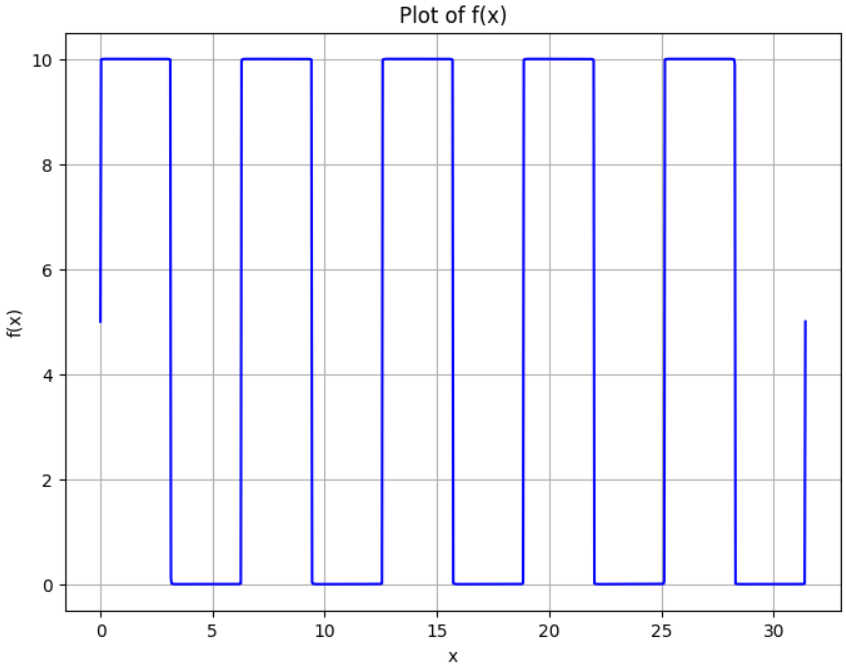
\includegraphics[width=\columnwidth]{sections/1_plot.png}
  \caption{Plot Generated Using Calculated Fourier Series Expression}
\end{figure}

\subsection{Magnitude Spectrum of $C_k$}
The magnitude spectrum is obtained by computing $|C_k|$ for different values of $k$. It provides insight into how much of each frequency component is present in the signal:
\begin{equation}
    |C_k| = \sqrt{\operatorname{Re}(C_k)^2 + \operatorname{Im}(C_k)^2}.\\
\end{equation}
The magnitude spectrum plots $|C_k|$ against $k$.

For the given input wave, $|C_k|$ is 
\begin{equation}
    |C_k| =\frac{5}{\pi k}\left(\sqrt{2(1-cos(2\pi k\alpha)} \right)
\end{equation}

\begin{figure}[H]
  \centering
  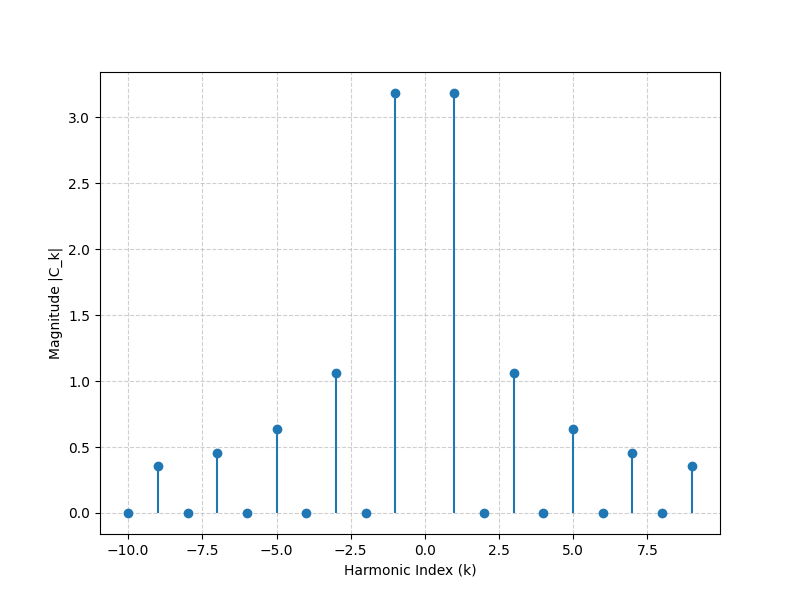
\includegraphics[width=\columnwidth]{sections/1_spectrum.png}
  \caption{For alpha=0.5}
\end{figure}
\begin{figure}[H]
  \centering
  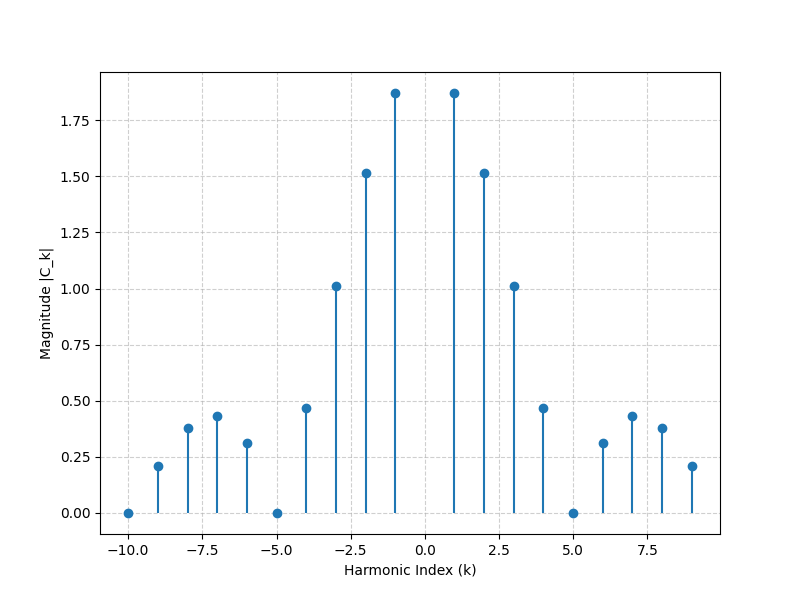
\includegraphics[width=\columnwidth]{sections/1_spectrum2.png}
  \caption{For alpha=0.2}
\end{figure}
\begin{figure}[H]
  \centering
  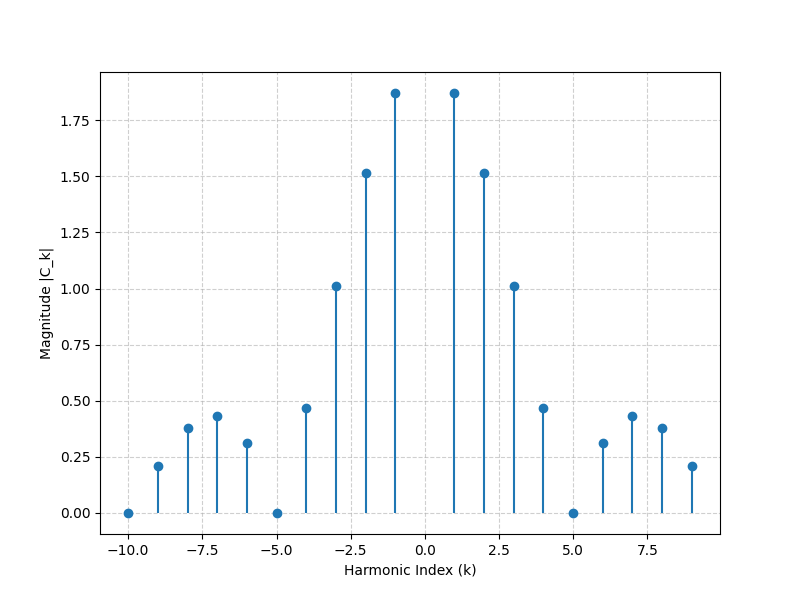
\includegraphics[width=\columnwidth]{sections/1_spectrum3.png}
  \caption{For alpha=0.8}
\end{figure}

\end{multicols}
